\section{Marco Teórico}

    \subsection{Redes Neuronales Artificiales}
    	
    	
        Las redes neuronales artificiales (RNA) son procesos los cuales contienen simples
        unidades de procesamientos. \\
        
        Como se puede observar, al mencionar RNA lo primero que se viene a la mente es el 
        procesamiento biol\'ogico por el que transita el cerebro humano. El m\'etodo principal 
        de las redes neuronales es sacarle el máximo poder a los algoritmos de aprendizaje 
        m\'aquina, ya que las redes neuronales tienen un antecedente biol\'ogico.\\

        Una red de una sola neurona solamente resuelve problemas lineales y tiene la 
        siguiente forma:
        \begin{figure}[H]
            \centering
            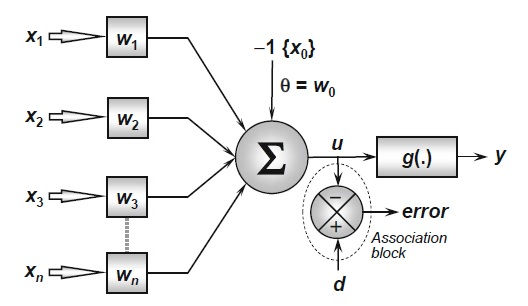
\includegraphics[width=\columnwidth]{ANN.jpg}
            \caption{Red Neuronal Artificial B\'asica}
            \label{fig:fig1}
        \end{figure}

        Donde
        $\begin{cases}  
            \Sigma
        \end{cases}$
        es la representaci\'on matem\'atica de la neurona. \\
        Los siguientes valores
        $\begin{cases}
            x_1, x_2, ... , x_n
        \end{cases}$
        señalando a 
        $\begin{cases} \label{eqn: weight}
            w_1, w_2, ... , w_n 
        \end{cases}$ 
        son los datos de entrada que se le dan a la red.
        Cuando la información entra en la neurona ah\'i se procesan los datos, la operci\'on realizada 
        es una sumatoria ponderada de ellos, dicha ponderaci\'on es asignada a ella como se observa en la siguiente 
        ecuaci\'on \eqref{eqn: weight}
        Entonces la f\'ormula de la sumatoria quedar\'ia de la siguiente manera:
        $\begin{cases} \label{eqn: summation}
            w_1x_1 + w_2x_2 + w_3x_3
        \end{cases}$ \\
        Al verificar bien esta formula, se puede observar que se parece a la operaci\'on de una regresi\'on 
        la cual es:
        $\begin{cases}
            y = w_0 + w_x.
        \end{cases}$
        Internamente la neurona realiza una regresi\'on lineal, el parámetro que permite a la neurona 
        moverse verticalmente en la recta se conoce como sesgo, este valor se agrega a la conexi\'on, el cual \
        usualmente se le da un valor de 1. \\
        Agregando este nuevo valor a la f\'ormula, queda de la siguiente manera: \\
        $\begin{cases}
            w_1 + w_2 + w_3 + b
        \end{cases}$ 
        donde \textit{b} es el sesgo. \\
        
        Un inconveniente del uso de una sola neurona para experimentos es que solo 
        va a resolver ejercicios parecidos a la puerta l\'ogica AND u OR \label{sec: one neuron}.
        
        \begin{figure}[H]
            \begin{subfigure}[H]{0.49\textwidth}
                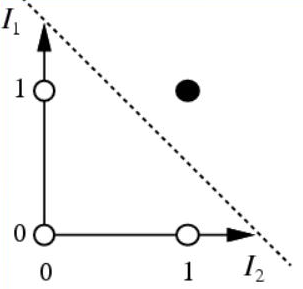
\includegraphics[width=\textwidth, height=\textwidth]{and.png}
                \caption{Puerta L\'ogica And}
                \label{fig:f2}
            \end{subfigure}
            \hfill
            \begin{subfigure}[H]{0.49\textwidth}
                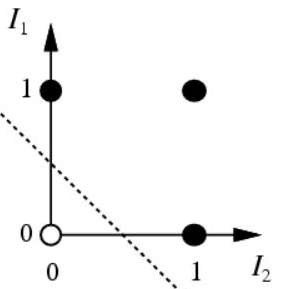
\includegraphics[width=\textwidth, height=\textwidth]{or.png}
                \caption{Puerta L\'ogica Or}
                \label{fig:f2}
            \end{subfigure}
            \caption{Puertas L\'ogicas \cite{mcmahon2014}}
        \end{figure}
        
        Pero problemas de tipo XOR no puede, ya que como se nota, una sola neurona sirve para 
        clasificar de un solo lado, así que no puede clasificar ejercicios
        como los de la Figura \eqref{fig:fig3}.

        \begin{figure}[H]
            \centering
            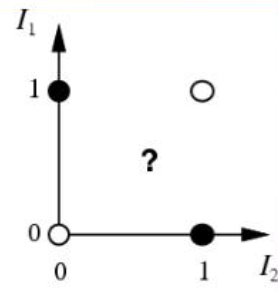
\includegraphics[width=5cm]{xor.png}
            \caption{Puerta L\'ogica Xor \cite{mcmahon2014}}
            \label{fig:fig3}
        \end{figure}

        Para solucionarlo se usan dos o m\'as neuronas, adem\'as de la funci\'on de activaci\'on.

            \subsubsection{Funci\'on de Activaci\'on} \label{sec: activation}
            
            
                Dicho m\'etodo se utiliza cuando el modelo de RNA contiene dos o m\'as neuronas.
                Esta funci\'on lo que provoca es dar al modelo una salida no lineal, para 
                eso la f\'ormula \eqref{eqn: summation} es distorcionada para quedar de la siguiente 
                manera: 
                $\begin{cases}
                    f( w_1x_1 + w_2x_2 + w_3x_3 )
                \end{cases}$
                En otras palabras esto es la suma de varias regresiones lineales, lo cual provoca que se obtenga 
                un resultado no lineal. \\
                
                Al hablar de funciones de activaci\'on se deben de comentar las m\'as comunes, como lo es la 
                funci\'on escalonada.
                
                \begin{figure}[H]
                    \centering
                    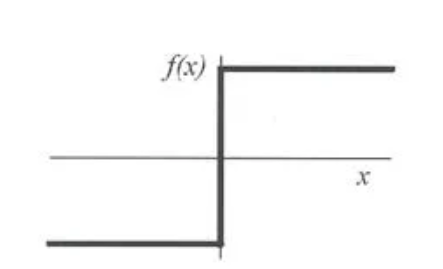
\includegraphics[width=5cm]{staggered.png}
                    \caption{Funci\'on Escalonada}
                    \label{fig:fig4}
                \end{figure}

                Dicha funci\'on es representada con: 
                
                \[f(x) = \left\{ \begin{array}{lr} 0 & : x < 0\\ 1 & : x \ge 0 \end{array} \right. \]

                La funci\'on sigmoidal, es una de las m\'as comunes, su forma es: 

                \begin{figure}[H]
                    \centering
                    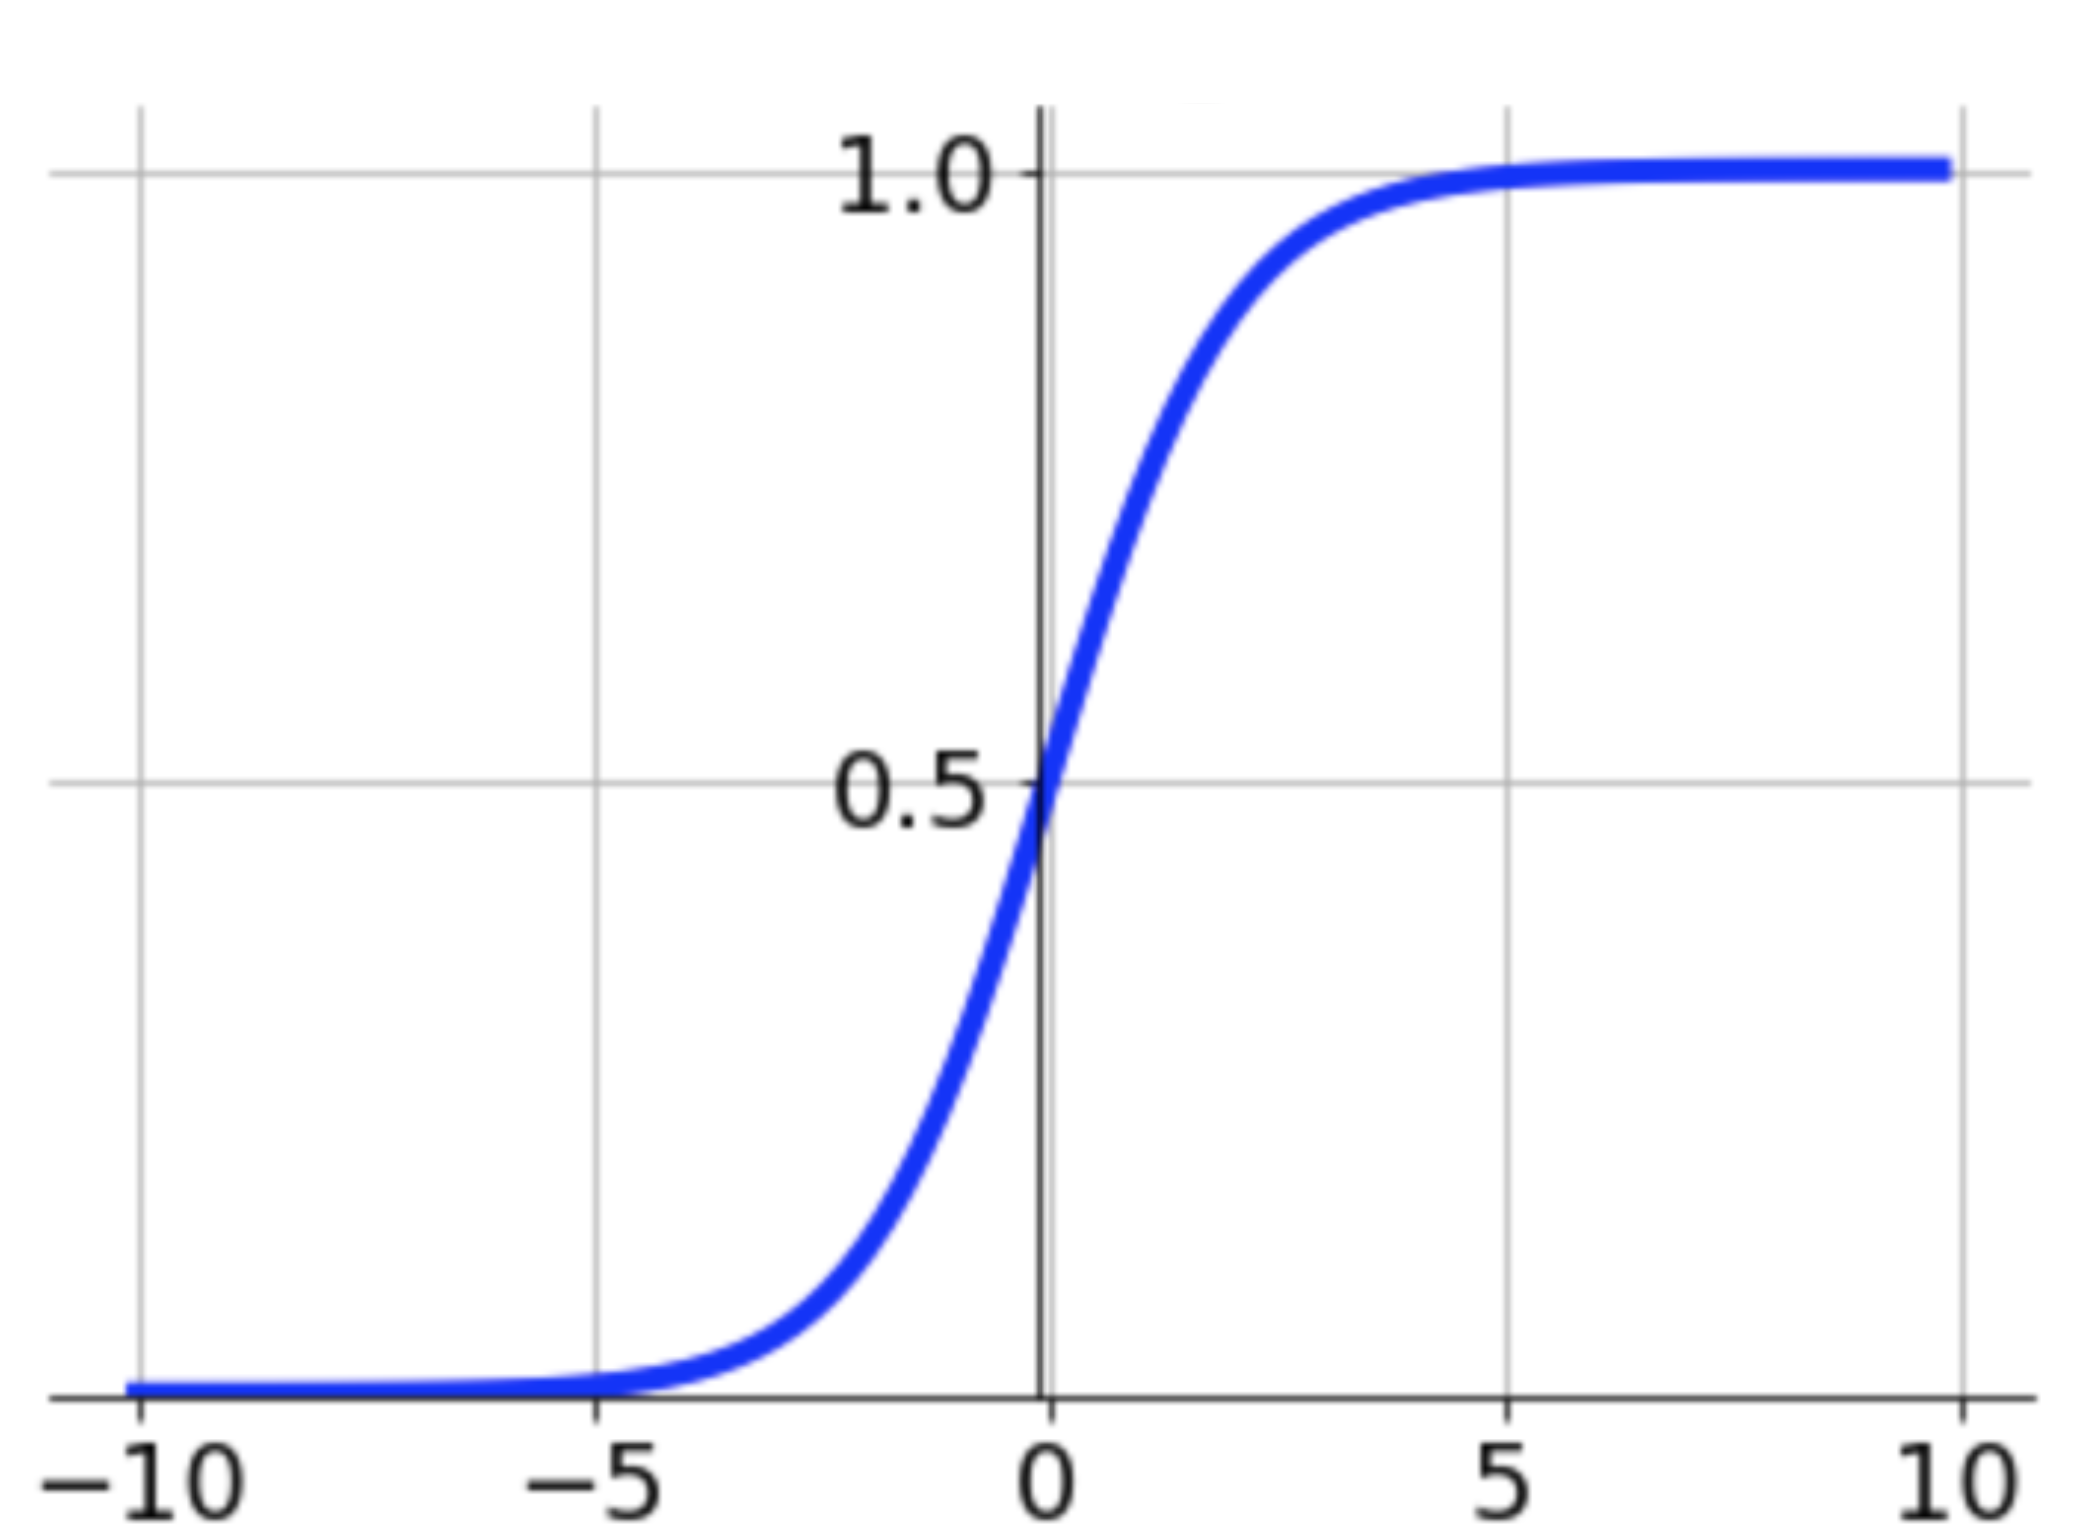
\includegraphics[width=5cm]{sigmoid.png}
                    \caption{Funci\'on Sigmoide}
                    \label{fig:fig5}
                \end{figure}

                La cual es representada por la siguiente formula:

                \[f(x) = \sigma(x) =  \left\{ \frac{1}{1 + e^{-x}} \right. \]

                Aparte de agregar deformaciones en la linea, ayuda en 
                cuestiones probabil\'isticas ya que se representa del rango de 0 a 1. \\

                La funci\'on de Unidad Rectificada Lineal o RELU, la cual es una funci\'on lineal
                que cuando es positiva es igual a 1 y cuando es negativa es constante a 0, su forma es: \label{subsec: relu}

                \begin{figure}[H]
                    \centering
                    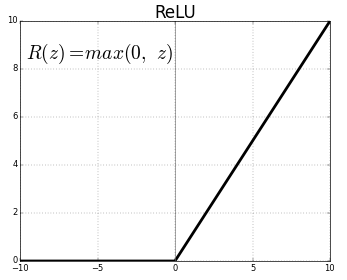
\includegraphics[width=6cm]{relu.png}
                    \caption{Funci\'on ReLU}
                    \label{fig:fig6}
                \end{figure}

                Se representa con la siguiente formula \cite{Freire2021}: 

                \[f(x) = \left\{ \begin{array}{lr} 0 & : x < 0\\ x & : x \ge 0 \end{array} \right. \]

                La función Softmax transforma las salidas a una representación en forma de 
                probabilidades, de tal manera que el sumatorio de todas las probabilidades 
                de las salidas de 1, su gr\'afica es: \label{subsec: softmax}

                \begin{figure}[H]
                    \centering
                    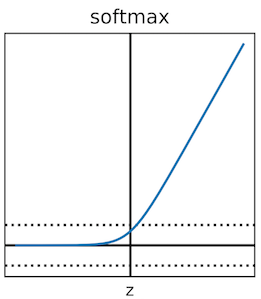
\includegraphics[width=6cm]{softmax.png}
                    \caption{Funci\'on Softmax}
                    \label{fig:fig7}
                \end{figure}

                Su representaci\'on matem\'atica es \cite{calvo-2018}:

                \[f(z)_j = \left\{ \frac{e^{z_j}}{\sum_{K=1}^{K} e^{z_k}} \right. \]

        Las redes neuronales presentan demasiadas utilidades las cuales ayudan a resolver problemas como los 
        siguientes \cite{liu2015}: no linealidad, mapeo entrada-salida, aprendizaje robusto 
        a errores en los datos de entrenamiento, entre otros.

        Existen varios tipos de Redes Neuronales tales como: Redes Neuronales de Perceptr\'on 
        Multicapa, Redes Neuronales Convolucionales, entre otras.
    
        \subsection{Redes Neuronales de Perceptr\'on Multicapa}
        
        Este tipo de redes entran en el paradigma de Aprendizaje Profundo, ya que como se explic\'o en 
            la secci\'on anterior \eqref{sec:delimitation}, aqu\'i la emulaci\'on de las neuronas humanas son m\'as 
            exactas.
            Adem\'as como se explica en esta sección \eqref{sec: one neuron} no es muy recomendado trabajar con una sola 
            neurona por los problemas de tipo XOR, que por lo general, es el que se presenta frecuentemente en las problemáticas.\\

            Dichas neuronas se dividen en tres capas: capa inicial, oculta y final. En las capas ocultas se pueden 
            tener m\'as de una fila de neuronas, estas son las encargadas de realizar las operaciones para eliminar 
            la linealidad de los proyectos. 

            En la secci\'on vista anteriormte \eqref{sec: activation} la linealidad se elimina con las funciones de activaci\'on, dicha funci\'on 
            es manipulable si se modifican los parámetros de la red, esto permitirá que se elabore un plano tridimencional, y con este plano se puede encontrar la soluci\'on al problema planteado.\\
            
            Como se puede observar en la siguiente imagen \eqref{fig:fig8} esta red est\'a
            construida por cuatro capas, la cual de ellas dos son ocultas, dentro de esas 
            capas es donde se realiza la ejecuci\'on de las funciones de activaci\'on. 
            Cada neurona de color azul va a generar una funci\'on (puede ser sigmoidal, escalonada, entre otras), 
            y cuando se llegue a la capa de salida, cada funci\'on se va a sumar, de esta manera 
            se obtendrá una funci\'on no lineal que de resoluci\'on al proyecto.

            \begin{figure}[H]
                \centering
                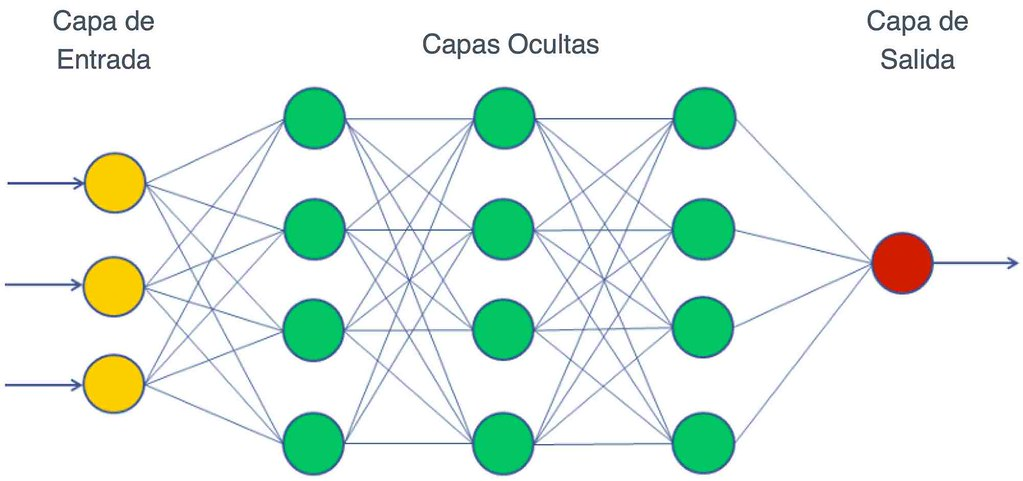
\includegraphics[width=\columnwidth]{multipercep.jpg}
                \caption{Perceptron Multicapa}
                \label{fig:fig8}
            \end{figure}

            
        \subsection{Algoritmo Backpropagation}
        	
        	
        	El bacpkpropagation es el algoritmo donde se explica c\'omo aprende la red.
            Dicho algoritmo fue presentado en 1986, lleg\'o a resolver el problema del perceptron 
            ya que ten\'ia muchas limitaciones, lo que provoc\'o que varios experimentos de inteligencia
            artificial se pararan.\\

            Este algoritmo permite que la red aprenda por si sola, en 1986 se present\'o \cite{rumelhart1986}, 
            donde muestran un nuevo algoritmo el cual permite que una red neuronal pueda auto-ajustar todos sus 
            parámetros para aprender una representaci\'on interna de la informaci\'on que se esta procesando.\\

            Usando este algoritmo se podrá obtener las derivadas parciales del gradiente y del peso, las cuales
            sirven para la optimizaci\'on de la red neuronal, dichas derivadas son:
            \begin{equation*}
                \frac{\partial C}{\partial W^L}
            \end{equation*}
            
            Pero no se debe de olvidar que también se debe de calcular las derivadas del sesgo, la derivada anterior
            queda de la siguiente forma:
            \begin{equation*}
                \frac{\partial C}{\partial b^L}
            \end{equation*}
            donde \textit{L} pertenece al n\'umero de capa donde se encuentra. \\
            
            Lo que permite a este algoritmo encontrar el error de la derivada es la \textit{chain rule}, la cual en resumen 
            da la siguiente ecuaci\'on :
            \begin{equation*}
                C(a(Z^L))
            \end{equation*}

            Donde 
            $\begin{cases}
                Z^L
            \end{cases}$
            representa el resultado de la suma ponderada, y la forma explicita de Z es:
            \begin{equation*}
                Z^L = W^LX + b^L
            \end{equation*}
            \textit{a} es la funci\'on de activaci\'on 
            y \textit{C} es la funci\'on de Coste.

            Al aplicar la \textit{Chain Rule} se obtiene que las derivadas parciales a conseguir son:
            \begin{equation*}
                \frac{\partial C}{\partial w^L} = \frac{\partial C}{\partial a^L} \cdot \frac{\partial a^L}{\partial z^L} \cdot \frac{\partial z^L}{\partial w^L} 
            \end{equation*}
            \begin{equation*}
                \frac{\partial C}{\partial b^L} = \frac{\partial C}{\partial a^L} \cdot \frac{\partial a^L}{\partial z^L} \cdot \frac{\partial z^L}{\partial b^L}
            \end{equation*}
            \\

            Como se observa, el uso de todas estas derivadas parciales permiten encontrar el error, en otras palabras, lo que realiza dicho algoritmo es terminar un proceso, si se encuentra un error, este va a regresar
            hasta la neurona que da error, pero regresa cambiando el valor de \textit{w}, este proceso se va a 
            repetir hasta encontrar el error perfecto, el cual es donde el error disminuye a lo m\'as bajo y el resultado
            de la red es lo m\'as acertado.\\

            Con lo anterior expuesto, se puede decir
            que esta metodolog\'ia es muy \'util en el uso de redes neuronales, es por eso que 
            se usa en la investigaci\'on \cite{bullinaria2009}, para obtener un buen resultado
            en el aprendizaje incremental, como es explicado ah\'i es usado para que las redes obtengan una buena topolog\'ia con 
            buena actualizaci\'on de pesos.

        \subsection{Redes Neuronales Convolucionales}
        	
        	
            Las redes neuronales convolucionales (RNC) son las que facilitan el reconocimiento de imágenes, el trabajo de reconocimiento de
            imágenes se puede elaborar con RNAs, pero esta tiene demasiadas desventajas, como lo que es p\'erdida de datos, porque cuando se 
            ingresa una imagen a la capa de entrada, esta se debe de convertir en vectores, si la imagen es de 100 pixeles por 100 pixeles
            se tendrá un vector de 10000 pixeles, esto solo ser\'a en imágenes a blanco y negro, si la imagen es del mismo tamaño pero a color
            se obtendrá un vector de 30000 pixeles, ya que se usan los filtros RGB (Rojo, Verde, Azul).

            Estas redes, presentan una soluci\'on para la problemática mencionada anteriormente, se basan en las conexiones que existen en 
            el cerebro junto a la de los ojos.

            Sus capas se distribuyen como se muestra Figura \eqref{fig:fig9}:
            
            
            \begin{figure}[H]
                \centering
                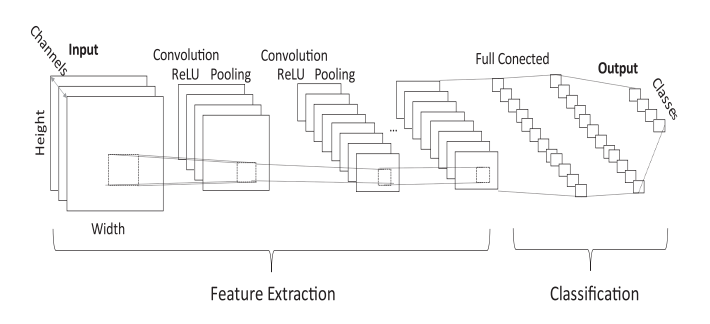
\includegraphics[width=\columnwidth]{CNN architecture.png}
                \caption{Arquitectura de una RNC \cite{Ortiz2020}}
                \label{fig:fig9}
            \end{figure}

            La capa de entrada contiene una matriz o tensor de matriz (m\'as de una matriz), las capas ocultas con dos etapas, y la 
            capa de salida, donde se obtendrá el resultado de la predicci\'on. \\
            
            La primer etapa es de extracci\'on de características, donde las capas están unidas a capas de \textit{pooling}, estas capas son 
            donde la imagen se divide en distintos kernels (filtros) el cual permitirá hacer submatrices a las imágenes y así poder recrearla
            en otra matriz, estos filtros deben ser menor de la imagen, se pueden tener m\'as de un kernel para
            analizar bien la imagen, existen dos m\'etodos de \textit{pooling}: el \textit{Max Pooling} y el \textit{Average Pooling},
             el \textit{Max Pooling} extrae el valor m\'aximo de las submatrices para crear otra matriz, como se puede observar en la 
            Figura \eqref{fig:fig10}, mientras que el \textit{Average Pooling} el cual obtiene el promedio de las submatrices y con 
            estos promedios genera otra matriz, como se puede ver en la Figura \eqref{fig:fig10} para un mejor resultado se tiene una capa de extracci\'on 
            o de convoluci\'on con otra capa de pooling, se pueden tener tantas capas de convoluci\'on como las de pooling 
            para tener una mejor abstracci\'on de conocimientos, en este tipo de conexiones se usan las funciones de activaci\'on conocidas como Relu \eqref{subsec: relu}. 

            \begin{figure}[H]
                \begin{subfigure}[H]{0.49\textwidth}
                    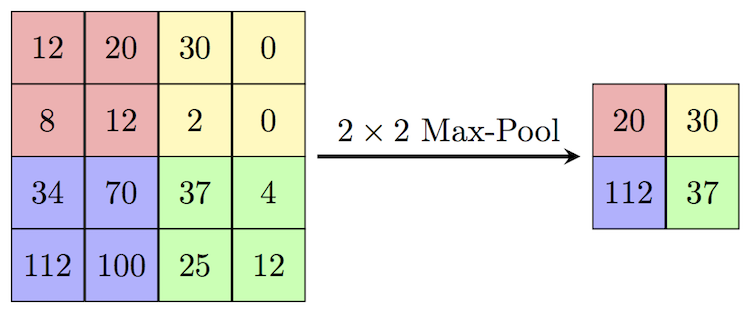
\includegraphics[width=5cm, height=3cm]{Maxpool.png}
                    \caption{Max Pooling}
                    \label{fig:fig10}
                \end{subfigure}
                \hfill
                \begin{subfigure}[H]{0.49\textwidth}
                    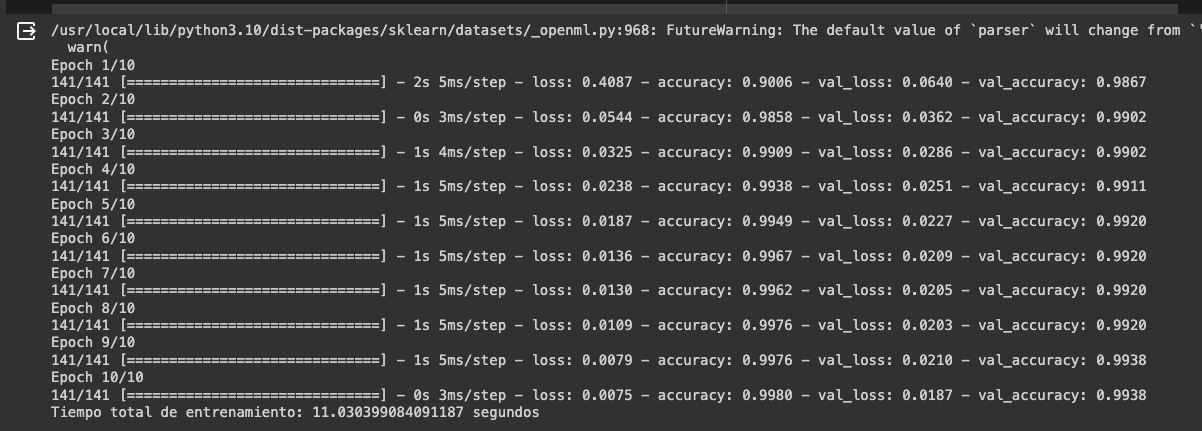
\includegraphics[width=5cm, height=3cm]{averagePooling.png}
                    \caption{Average Pooling}
                    \label{fig:fig10}
                \end{subfigure}
                \caption{M\'etodos Pooling}
            \end{figure}

            La segunda etapa es la de Full Conected, que equivale a tener una red normal o en otras palabras tener una RNA, aqu\'i 
            es donde el modelo va a predecir que es lo que se presenta, puede decir si en la imagen hay un perro, gato o alg\'un mueble, 
            para eso la funci\'on de activaci\'on que se usa es softmax \eqref{subsec: softmax}, la cual se maneja con probabilidad, esto
            permitirá que se obtenga una buena probabilidad de lo que se puede obtener por la capa de entrada \cite{duran2017,Ortiz2020}.\\
  

\subsection{Aprendizaje}

    \subsubsection{Aprendizaje en humanos}
    	
    	
        El humano tiene una forma de aprendizaje muy particular, la cual se basa del estudio, donde lee, escribe y practica acerca de
        su tema de interés, pero dicho aprendizaje se puede ir olvidando, esta es una acción muy común que a cualquier persona le sucede.
        Existen estudios donde se comenta que existen tres motivos del porque se olvidan las cosas, proviene parte de la regularización de las emociones,
        el como se adquirieron los conocimientos, y porque el olvido es un proceso por el cual el ser humano transita a lo largo de su vida \cite{Nrby2015}. Pero cabe
        mencionar que esto no es lo único que causa la perdida de memoria, ya que existe la déficit de memoria. 

    \subsubsection{Aprendizaje Humano}
    	
    	
        Al momento de hablar del aprendizaje humano, se debe de hablar de la ciencia cognitiva, que es quien se encarga de descubrir esta incógnita,
        esta ciencia lo estudia de un modo multidisciplinario, el cual abarca las \'areas de \cite{bransford2000}: antropología, lingüística, 
        filosofía, sicología del desarrollo, ciencia de la computación, neurociencia.
        Con el método de esta ciencia se pueden descubrir dos tipos de aprendizaje que son: el aprendizaje con compresi\'on y el aprendizaje Activo.
        
        \subsubsection{Aprendizaje con Comprensi\'on}
        	
        	
            La comprensi\'on es una actividad la cual se ha generado al momento de realizar cualquier tipo de lectura.\\
            
            Teniendo un enfocamiento en el \'ambito estudiantil, ya que es donde m\'as se maneja esta t\'actica, esto es una
            practica algo compleja, sistemática y organizada, pues da el significado de la literatura y durabilidad del aprendizaje.
            Al conocer esto se puede decir con seguridad que para cualquier tipo de aprendizaje la comprensi\'on es 
            una parte primordial \cite{perez2014}.

        \subsubsection{Aprendizaje Activo}
        	
        	
            El aprendizaje de la forma en la que se conoce no es del todo efectiva, ya que el sistema educativo
            no se basa en el principio de \textit{belongingness}, el cual esta asociado al estimulo con su respuesta,
            y esto es lo m\'as importante para que el ser humano pueda aprender cualquier cosa.\\
            
            Este tipo de aprendizaje se basa en la recepci\'on de conocimientos y la pr\'actica donde se ponen en marcha los conocimientos adquiridos.\\
            Otro concepto importante aqu\'i es la tautolog\'ia doble (\textit{selbstt\"atiges Lernen}), que en palabras informales es convertirse en autodidacta, 
            se puede observar que esto pertenece a dicho aprendizaje, porque usa el principio mencionado anteriormente \cite{Huber2008}.

 \subsubsection{Aprendizaje Incremental}
 	
 	
 	Con el pasar de los años la tecnología a evolucionado, eso quiere decir que el Aprendizaje Automático se ha actualizado y que la 
        cantidad de datos va aumentado con más frecuencia.
        
        Se puede verificar como \textit{"Una tarea de aprendizaje es incremental si los ejemplos de entrenamiento usados para 
        resolverla están disponibles en horas extras, generalmente uno a la vez"} \cite{GiraudCarrier2000}, si los resultados no se 
        necesitan de manera urgente, este tipo de trabajos serán resueltos por algoritmos de aprendizaje no incremental. 

        Una área donde esto es de mucha utilidad es la \textit{Rob\'otica} porque este necesita estar en constante entrenamiento \cite{GiraudCarrier2000}.

        Dicha forma de aprender fue inspirada en la forma en que el humano aprende y esta más rápida, fue por esto que fue adoptada 
        por el aprendizaje m\'aquina.

        Con el paso del tiempo se ha convertido en un paradigma del aprendizaje automático, aquí el aprendizaje toma el lugar de nuevos ejemplos para juntarlos 
        y conforme van aprendiendo estos toman el lugar de los ejemplos ya aprendidos \cite{liu2015}.

        \subsubsection{Algoritmos de Aprendizaje Incremental}
        	
        	
        El algoritmo de aprendizaje incremental puede definirse como aquel que cumple los siguientes criterios:  
        1) Ser capaz de aprender y actualizarse con cada nuevo dato etiquetado o no etiquetado. 
        2) Conservar los conocimientos adquiridos previamente.
        3) No debe requerir el acceso a los datos originales. 
        4) Generar una nueva clase o cluster cuando sea necesario. Dividir o fusionar los clusters cuando sea necesario. 
        5). Ser de naturaleza dinámica con el entorno cambiante \cite{Deshmukh2013}.
        
        \begin{figure}[H]
        	\centering
        	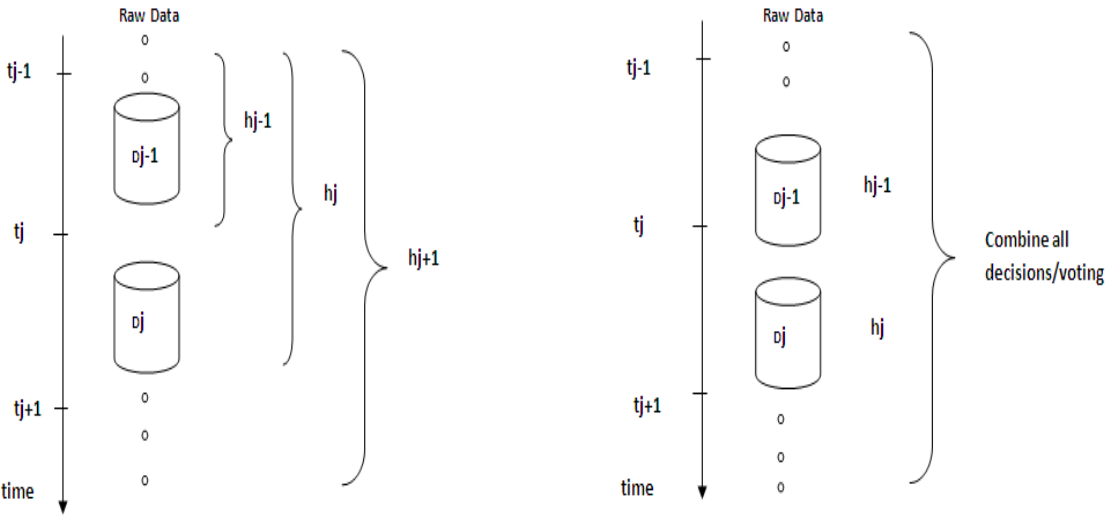
\includegraphics[width=\columnwidth]{MetodosAprendizajeIncremental.png}
            \caption{Dos enfoques tradicionales del aprendizaje incremental \cite{Deshmukh2013}.}
            \label{fig:fig11}
        \end{figure} 
        1 Metodología de acumulación de datos. 2 Metodología de aprendizaje por conjuntos.\\
        
		Como se observa en la Figura 11, en el primer método, cuando se recibe una nueva porción de datos Dj, se descarta hj-1 y se desarrolla una nueva hipótesis hj, basada en todos los datos disponibles acumulados hasta el momento. 
		Y en el segundo método, cuando se recibe una nueva porción de datos Dj, se desarrolla una única hipótesis nueva o un conjunto de hipótesis nuevas basadas en los nuevos datos. 
		Por último, se puede utilizar un mecanismo de votación para combinar todas las decisiones de las diferentes hipótesis y obtener la predicción final.\\
		
		Por ejemplo, si se deja que Dj-1 represente la porción de datos recibida entre el tiempo tj-1 y tj, y que la hipótesis hj-1 se desarrolle sobre Dj-1.\\
		El sistema aprenderá información de forma adaptativa cuando se reciba una nueva porción de datos Dj.	
		En el método de aprendizaje por conjuntos, se desarrolla una nueva hipótesis hj o un conjunto de hipótesis H:h1, i1,2,...,M, basadas en los nuevos datos.  
		A continuación, se utiliza el mecanismo de votación para combinar todas las decisiones de las diferentes hipótesis y llegar a la predicción final.
		La mayor ventaja de este enfoque es que no se requiere almacenar los datos vistos anteriormente, el conocimiento se ha almacenado en la serie de hipótesis desarrolladas a lo largo de la vida de aprendizaje.\\
		
			Conocimiento en el momento t: \\
			Dt es un trozo de datos con n instancias (i=1,...,n) \\
			(xi,yi) es una instancia en el espacio de características m-dimensional X\\ 
			Yi $\in$ Y ={1,...,K} clases \\
			Función de distribución Df \\
			Una hipótesis ht, desarrollada por los datos basados en Dt con Pt \\
			La nueva entrada estará disponible en el momento (t+1) \\\\
			
			Algoritmo de aprendizaje:\\
			\begin{enumerate}
				\item Encontrar la relación entre Dt y Dt+1
				\item Actualizar la función de distribución inicial Dt+1
				\item Aplicar la hipótesis ht a Dt+1 y calcular el pseudoerror de ht
				\item Refinar la función de distribución para Dt+1
				\item Se desarrolla una hipótesis por los datos basados en Dt+1 con Pt+1
				\item Repetir el procedimiento cuando se reciba la siguiente porción del nuevo conjunto de datos.
			\end{enumerate}
			Resultado: La hipótesis final.\\
		  
		
		            
                   
        
            \textit{"Un algoritmo de aprendizaje es incremental si,
            para cualquier muestra de entrenamiento dada:
            \begin{equation}
                e_{1} , .... , e_{s}
			\end{equation}
            produce un secuencia de hipótesis 
            \begin{equation}
                h_{0} , h_{1}, . . . , h_{n} 
            \end{equation}
            tal que hi+1 depende solo de hola(Tengo duda con la palabra hola si lo tradujiste fijate bien que hayas copiado bien, luego los simbolos no los copia como es ) y del ejemplo actual e"} \cite{GiraudCarrier2000}, como se 
            observa, estos son algoritmos que permiten a la inteligencia artificial poder realizar actividades de predicci\'on 
            de una manera m\'as eficaz.\\
            
            Un ejemplo del uso de esta rama es el proyecto \textit{COBWEB}, donde se trata de categorizar el n\'umero de Cl\'uster y la pertenencia 
            de dichas categor\'ias por medio de una m\'etrica probabil\'istica global, esto lo realiza por medio de que se agrega 
            una nueva categor\'ia, este proceso lo que realizar\'a es actualizar todas las probabil\'isticas con los nuevos datos recabados \cite{fisher1987}.

